%!TEX TS-program = xelatex
\documentclass[]{friggeri-cv}
\usepackage{afterpage}
\usepackage{hyperref}
\usepackage{color}
\usepackage{xcolor}
\usepackage{smartdiagram}
\usepackage{fontspec}
% if you want to add fontawesome package
% you need to compile the tex file with LuaLaTeX
% References:
%   http://texdoc.net/texmf-dist/doc/latex/fontawesome/fontawesome.pdf
%   https://www.ctan.org/tex-archive/fonts/fontawesome?lang=en
%\usepackage{fontawesome}
\usepackage{metalogo}
\usepackage{dtklogos}
\usepackage[utf8]{inputenc}
\usepackage{tikz}
\usetikzlibrary{mindmap,shadows}
\hypersetup{
    pdftitle={},
    pdfauthor={},
    pdfsubject={},
    pdfkeywords={},
    colorlinks=false,           % no lik border color
    allbordercolors=white       % white border color for all
}

\smartdiagramset{
    bubble center node font = \footnotesize,
    bubble node font = \footnotesize,
    % specifies the minimum size of the bubble center node
    bubble center node size = 0.5cm,
    %  specifies the minimum size of the bubbles
    bubble node size = 0.5cm,
    % specifies which is the distance among the bubble center node and the other bubbles
    distance center/other bubbles = 0.3cm,
    % sets the distance from the text to the border of the bubble center node
    distance text center bubble = 0.5cm,
    % set center bubble color
    bubble center node color = pblue,
    % define the list of colors usable in the diagram
    set color list = {lightgray, materialcyan, orange, green, materialorange, materialteal, materialamber, materialindigo, materialgreen, materiallime},
    % sets the opacity at which the bubbles are shown
    bubble fill opacity = 0.6,
    % sets the opacity at which the bubble text is shown
    bubble text opacity = 0.5,
}

\RequirePackage{xcolor}
\definecolor{pblue}{HTML}{0395DE}

\begin{document}
\header{Pietro}{Della Briotta Parolo}
      {Data Analyst/Scientist}
      
% Fake text to add separator      
\fcolorbox{white}{gray}{\parbox{\dimexpr\textwidth-2\fboxsep-2\fboxrule}{%
.....
}}

% In the aside, each new line forces a line break
\begin{aside}
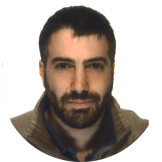
\includegraphics[scale=0.65]{img/foto.png}
  \section{Address}
    Ellipsipolku 4a,41
     02210 Espoo
    ~
  \section{Contacs}
   
\includegraphics[scale=0.03]{img/phone.png} +358505124297
   
\includegraphics[scale=0.03]{img/skype.png} dbp.pietro 
    
\includegraphics[scale=0.03]{img/mail.png} dbp.pietro@gmail.com 
~ 
  % use  \hspace{} or \vspace{} to change bubble size, if needed
  \section{Technical Skills}
    \smartdiagram[bubble diagram]{
        \textbf{Python},
        \textbf{Complex} \\\textbf{Systems},
         \textbf{Nework} \\\textbf{Theory},
        \textbf{SQL},
        \textbf{Statistics},
        \textbf{Big}\\ \textbf{Data}
    }
    ~
  \section{Personal Skills}
    \smartdiagram[bubble diagram]{
        \textbf{Team}\\\textbf{Player},
        \textbf{Initiative},
        \textbf{Curiosity},
        \textbf{Problem}\\\textbf{Solving},
        \textbf{Organize}
    }
    ~
    \section{OS Preference}
    \textbf{GNU/Linux}
\includegraphics[scale=0.40]{img/5stars.png}
    \textbf{Unix}
\includegraphics[scale=0.40]{img/4stars.png}
    \textbf{Windows}
\includegraphics[scale=0.40]{img/4stars.png}
    ~
  \section{Languages}
    \textbf{Italian}
\includegraphics[scale=0.40]{img/5stars.png}
    \textbf{English}
\includegraphics[scale=0.40]{img/5stars.png}
    \textbf{German}
\includegraphics[scale=0.40]{img/3stars.png}
    \textbf{Finnish}
\includegraphics[scale=0.40]{img/3stars.png}
    \textbf{Hungarian}
\includegraphics[scale=0.40]{img/1stars.png}
    ~
\end{aside}

\section{Education}
\begin{entrylist}
\unientry
{2017-}
{Bioinformatician}
{0.06}
{img/FIMM.png}
{University of Helsinki}
{I am a member of the genetic analysis team in the Finngen project, which aims to genotype 500 000 Finns and couple the genetic data with health registry data of each participant. These activities will contribute to a reference database used in rare variant studies, powerful phenome-wide association studies elucidating genetic basis of health and disease and eventually hopefully as a step in realizing the promise of personalized medicine in the future.}
\\

  \aaltoentry
    {2013 - 2017}
    {PhD in Computer Science}
{img/cs.png}
{img/Aalto_logo.png}
{Aalto University}
{During my PhD studies I've been mainly focused on the statistical analysis of large data sets, with a particular interest in
scientific data stemming from published publications. My focus has been on the analysis of how the structure of science and
the key statistical properties of individual publications have been changing in time due to the constant growth of scientific
literature.\\
Thesis: Analysis of cumulative and temporal patterns in science
}
\\

\unientry
    {2010 - 2012}
    {Masters's Degree in Pyshics of Complex Systems}
    {0.1}
   {img/turin.png}
    {Turin University}
    {During my masters I studied the application of methods of physics in multidisicplinary fields, with a particular focus
    to socio-economical ones (Econophysics,Agent Based Models, Game Theory, Network Theory, Social Networks, Epidemiology) and to biological ones
    (Neural Networks, Genetics). I also visited Prof. Dirk Helbing's group in Z\"urich for 6 months.\\
     Thesis: Undermining the Wisdom of Crowds: Effects of Social Influence in a Network of Communities,
}
\\
\unientry
    {2006 - 2010}
    {Bachelor Degree in Physics}
    {0.3}
    {img/unipv.png}
    {Pavia University}
{ Thesis: 20 years of cold fusion.}


\end{entrylist}





\section{Publications}

 Pietro Della Briotta Parolo, Mikko Kivel\"a, Kimmo Kaski\\
\textbf{On the Shoulders of
Giants: tracking the cumulative knowledge spreading in citation networks.}
\emph{prepint}
\\
P. Della Briotta Parolo, R. K. Pan, R. Ghosh, B. H. Huberman
K. Kaski, S. Fortunato, \\
\textbf{On the decay of attention in science}, 
\emph {Journal of Informetrics, Volume 9, Issue 4,  Pages 734–745, October 2015}
\\
F. Becattini, A. Chatterjee, S. Fortunato, M. Mitrović, R. K. Pan, P.
Della Briotta Parolo,
\textbf{Growing time lag threatens Nobels}, 
\emph{Nature 508, 186 (2014)}.
\\

\section{Press Coverage}

The paper Growing time lag threatens Nobels (Nature 508, 186, 2014), by F. Becattini, A.
Chatterjee, S. Fortunato, M. Mitrović, R. K. Pan and P. Della Briotta Parolo, was featured in many
media sources and blogs, including:

\begin{itemize}
\item Le Figaro, http://www.lefigaro.fr/sciences/2014/10/08/01008-20141008ARTFIG00295-leslaureats-des-nobel-sont-de-plus-en-plus-ages.php
(October the 8th, 2014);
\item Der Spiegel, http://www.spiegel.de/wissenschaft/mensch/nobelpreis-dauer-zwischenzentraler-forschung-und-ehrung-waechst-a-963516.html
(April the 10th, 2014);
\end{itemize}

The paper \textit{On the decay of attention in science}, by P. Della Briotta Parolo, R. K. Pan, R. Ghosh, B. H. Huberman
K. Kaski, S. Fortunato was featured in media sources including:
\begin{itemize}
\item Der Spiegel,​ http://www.spiegel.de/wissenschaft/mensch/publikationsflut-forscher-veroeffentlichen-zu-viel-a-1022970.html
\item Daily Mail, ​http://www.dailymail.co.uk/sciencetech/article-2993954/Science-decay-studies-new-study-finds.html​
\end{itemize}


\section{Other Experience}

\begin{entrylist}

\work
{2015}
{Conference Organizer}
{0.05}
{img/iccss.png}
{I was part of the team that helped organize the first International Conference on Computational Social Science in 2015 in Helsinki, Finland. The event has since become a regular event in the world of Computation Social Science.
}
\\

\work
{2013 - now}
{Travel Organizer}
{0.1}
{img/anm.jpg}
{Avventure nel Mondo is an Italian association with promotes group travelling. It has almost 1000 destinations worldwide, for all ranges of customers, spacing from easy/fully booked trips to more intense "discovery" ones.

A tour coordinator is responsible of the organization of the trip before departure, mainly by contacting participants and handling the communication with local partners. During the trip, it is their responsibility to make sure all things run smoothly and safely, allowing the full enjoyment of the group experience.}


\end{entrylist}

\begin{aside}
  \section{Personal Interests}
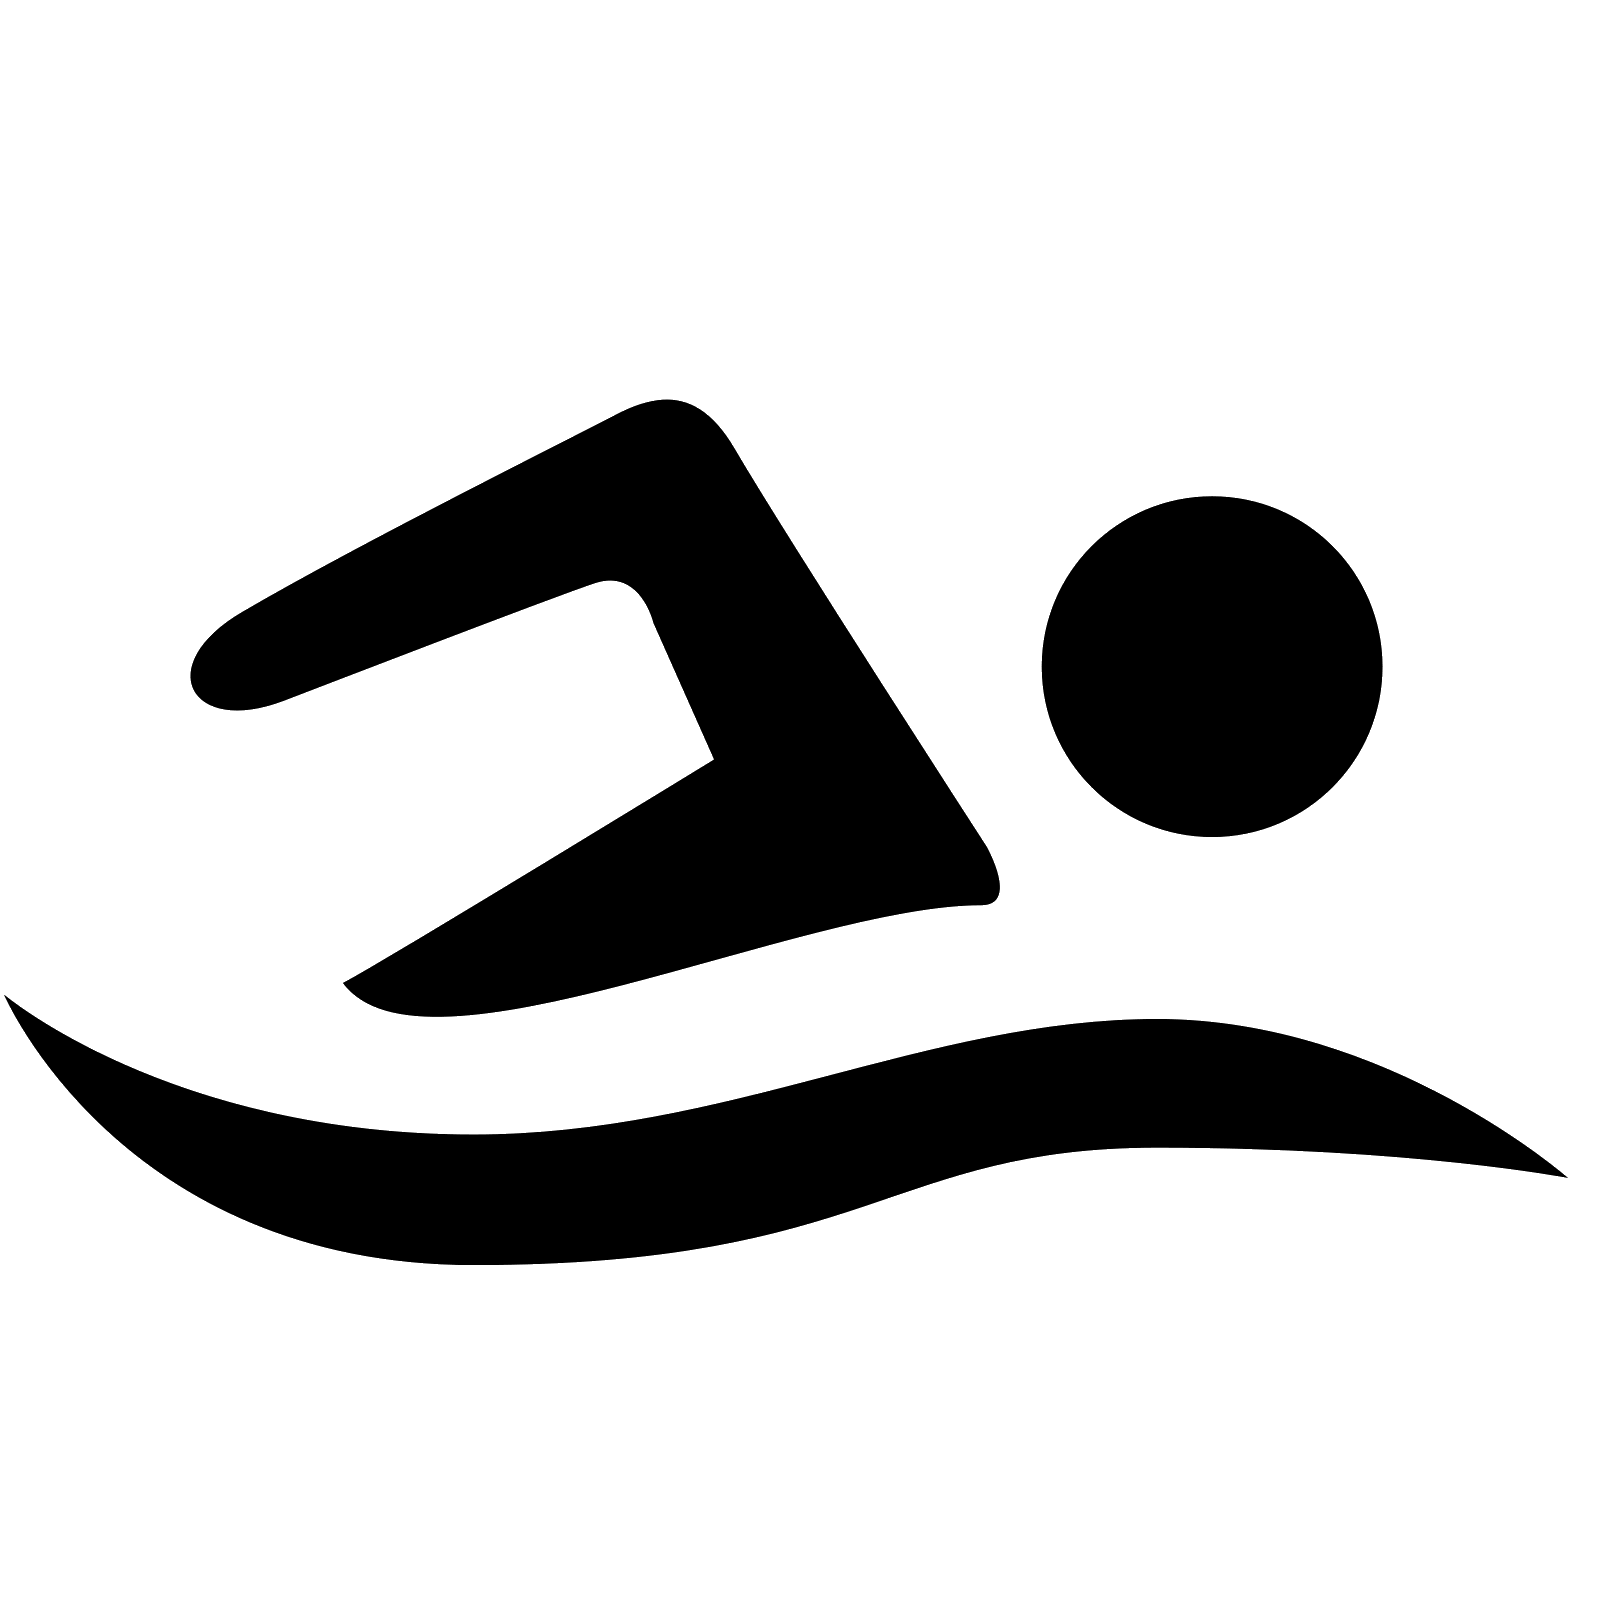
\includegraphics[scale=0.01]{img/swimming.png}
\includegraphics[scale=0.03]{img/kayak.png}
\includegraphics[scale=0.05]{img/tennis.png}
\includegraphics[scale=0.05]{img/running.png}
\end{aside}

\end{document}
